\subsection{Bild speichern im Backend}
Hauptgrund für die schlussendliche Nichtimplementierung des optionalen Speicherns von Bilder zu Fragen war vorallem
die Zeiteinteilung, da das Anliegen für das Einbinden von Bildern erst kurz vor Abgabe der Arbeit aufgekommen ist.
Trotz dessen wurden Versuche für die Speicherung im Backend unternommen. Diese wurden jedoch im weiteren Verlauf
eingestellt.
\newline
\newline
Um ein Bild in der Datenbank zu speichern, kann ein Objekt von Typ byte[] erstellt werden. (Siehe: \ref{lst:lob})
\begin{lstlisting} [caption= @Lob, label=lst:lob]
    @Lob
    @Column(name = "photo")
    private byte[] photo;
\end{lstlisting}
Das übergebene Bild muss in ein byte[] umgewandelt werden, um dieses zu speichern.
Um dies zu erreichen, wurden folgende Versuche unternommen:

\subsubsection{Bild in Byte Array umwandeln}
Beim ersten Versuch wurde das Bild mithilfe eines ImageIO.read() gelesen und mit einem ByteArrayOutputStream
in einem Array gespeichert. Danach wurde das Array durch einen ByteArrayInputStream eingelesen und mit
ImageIO.write() im File output.jpg gespeichert.

\begin{lstlisting} [caption=Bild in Byte Array umwandeln, label=lst:ImageToByteArray]
    public void saveImage(File imageFile){
       BufferedImage bImage = null;
        try {
            bImage = ImageIO.read(imageFile);
        } catch (IOException e) {
            e.printStackTrace();
            System.out.println(e.getMessage());
        }
        ByteArrayOutputStream bos = new ByteArrayOutputStream();
        try {
            ImageIO.write(bImage, "jpg", bos );
        } catch (IOException e) {
            e.printStackTrace();
        }
        byte [] data = bos.toByteArray();
        Question question = new Question("hallo", data, 100, QuestionType.FREETEXT,null);
        save(question);
    }

    public File returnImage(byte[] data){
        ByteArrayInputStream bis = new ByteArrayInputStream(data);
        BufferedImage bImage2 = null;
        try {
            bImage2 = ImageIO.read(bis);
        } catch (IOException e) {
            e.printStackTrace();
        }
        try {
            ImageIO.write(bImage2, "jpg", new File("output.jpg") );
        } catch (IOException e) {
            e.printStackTrace();
        }
        File imageFile = new File("output.png");
        return imageFile;
    }
\end{lstlisting}

\subsubsection{Bild mit Session in DB speichern}
Beim zweiten Versuch wurde mithilfe von HibernateUtil.getSessionFactory().openSession() eine Session eröffnet,
in der mittels eine FileInputStream das Bild in ein byte[] ungewandelt wird. Danach wird das erzeugte byte[] 
in der DB gespeichert. Um das byte[] aus der DB zu laden und in ein File umzuwandeln, verwendet man den
FileOutputStream.
\newline
\newline
Dieser Versuch wurde anfangs mit einem Bild, das lokal auf dem Rechner liegt, getestet. Dabei wurde das Bild
in der DB gespeichert und wieder geladen. Als ausporbiert wurde, ob dieser Versuch funktioniert, wenn das Bild
vom Frontend mitgesendet wird, trat der Fehler auf, dass man ein mitgeschicktes File nicht so leicht umwandeln kann.
Nach dieser Erkenntnis wurde auch dieser Versuch eingestellt.

\begin{lstlisting} [caption=Bild mit Session in DB speichern, label=lst:imageSessionSave]
public static void main( String[] args )
    {
        System.out.println("Hibernate save image into database");
        Session session = HibernateUtil.getSessionFactory().openSession();
        
        session.beginTransaction();
        
        //save image into database
        File file = new File("C:\\mavan-hibernate-image-mysql.gif");
        byte[] bFile = new byte[(int) file.length()];
        
        try {
         FileInputStream fileInputStream = new FileInputStream(file);
         //convert file into array of bytes
         fileInputStream.read(bFile);
         fileInputStream.close();
        } catch (Exception e) {
         e.printStackTrace();
        }
        
        Avatar avatar = new Avatar();
        avatar.setImage(bFile);
        
        session.save(avatar);
        
        //Get image from database
        Avatar avatar2 = (Avatar)session.get(Avatar.class, avatar.getAvatarId());
        byte[] bAvatar = avatar2.getImage();
        
        try{
            FileOutputStream fos = new FileOutputStream("C:\\test.gif"); 
            fos.write(bAvatar);
            fos.close();
        }catch(Exception e){
            e.printStackTrace();
        }

        session.getTransaction().commit();
    }
\end{lstlisting}

\subsection{CORS Fehler}
Nach der Implementierung einiger Hauptfunktionen im Frontend -- zum Beispiel das Erstellen eines Fragebogen --
wurden diese mit den bereits erstellten REST-Methoden verbunden und getestet. Im Laufe der Testungen sind 
CORS Fehler aufgetreten. Wie so ein Fehler aussieht wird beispielhaft in Abb. \ref{fig:cors} dargestellt.
Ein CORS Fehler entsteht beim Laden von Daten aus verschiedenen Quellen. Das Problem wurde durch das Einfügen 
von folgender Zeile \ref{lst:CorsError} in den application.properties behoben.

\begin{figure}[H]
    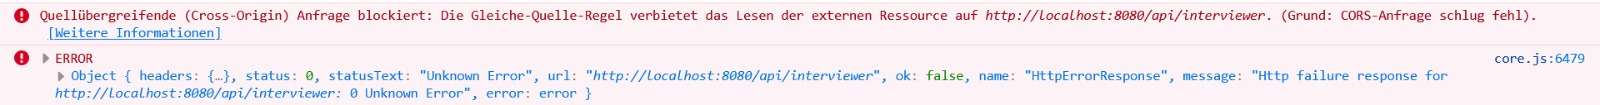
\includegraphics[width=1\textwidth]{pics/cors_error.jpeg}
    \centering
    \caption{CORS Fehler}
    \label{fig:cors}
\end{figure}

\begin{lstlisting} [caption=Lösung CORS Error, label=lst:CorsError]
    quarkus.http.cors=true
\end{lstlisting}

\subsection{Cyclic-Object-Error}
Cyclic-Object-Error (siehe Abb. \ref{fig:cycle} als Beispiel) können bei der Konvertierung von Angular-Objekten in 
JSON-Objekte auftreten. \cite{noauthor_typeerror_nodate}, \cite{noauthor_fixing_nodate}

Der Fehler tritt genau dann auf wenn:
\begin{enumerate}
    \item ein Objekt auf sich selbst referenziert
    \item zwei Objekte aufeinander referenzieren
    \item mehreren Objekten, die in einen Kreis aufeinander referenzieren, konvertiert werden sollen
\end{enumerate}

Das JSON-Format an sich unterstützt keine Objektreferenzen, daher versucht JSON.stringify() nicht, diese zu lösen, und schlägt entsprechend fehl. 
Veranschaulicht würde das JSON-Objekte unendlich lang und in die Tiefe gehen.
\begin{figure}[H]
  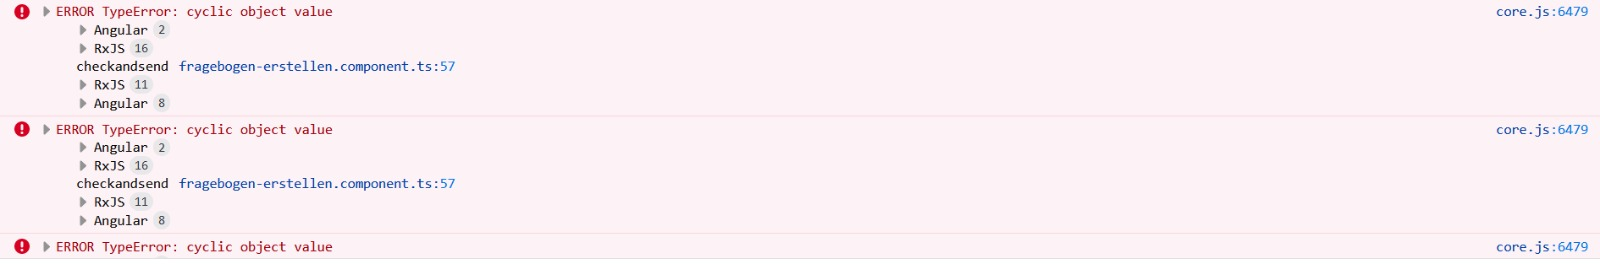
\includegraphics[width=1.2\textwidth]{pics/cycle_object.jpeg}
  \centering
  \caption{Cyclic-Object-Error}
  \label{fig:cycle}
\end{figure}
In der vorliegenden Arbeit wurde versehentlich ein Cyclic-Object erstellt, um die Darstellung von Fragen und zugehörigen
Antwortmöglichkeiten zu gewährleisten. Dabei referenzierte die Frage auf die Antwortmöglichkeit und die Antwortmöglichkeit auf die Frage.
Die Referenzierung der Antwortmöglichkeiten auf die Frage ist durch das Backend vorgegeben worden. Die Referenzierung der Antwortmöglichkeit auf die Frage 
wurde für die einfachere Zuordnung und Darstellung der beiden im Frontend eingefügt. (siehe Listing \ref{lst:alte Klassen mit cycle-error})
\begin{lstlisting}[language=TypeScript, caption=Klassen mit Cyclic-Error, label=lst:alte Klassen mit cycle-error]
import { Interviewer } from "./interviewer";
import { AnswerOption } from "./answer-option"

export class Questionnaire {
  constructor(
    public id = 0, public name :string = "", 
    public description : string = "", 
    public isPublic: Boolean = false, 
    public interviewer : Interviewer = new Interviewer(1, "HTL Leonding"),
    public AnswerOptions : AnswerOption[] = []
    ){}
}

import { Question } from "./question";

export class AnswerOption {
    constructor(
      public id = 0, public text :string = "", 
      public value = 0, 
      public sequenceNumber = 0, 
      public isCorrectAnswer = true, 
      public question : Question = new Question()
    ){}
}
\end{lstlisting}
Für die Übertragung von Daten zwischen Frontend und Backend wurde beschlossen JSON zu verwenden.
Dieses Format kann diese Referenzierung nicht darstellen und die einmalige Verwendung von
cycle.js, einer Bibliothek, die solche Referenzierung darstellen kann, wäre zu aufwändig gewesen.
\newline
\newline
Für die Lösung dieses Problem wurde eine neue Klasse erstellt und beide Objekte (Frage und Antwortmöglichkeiten-Liste) 
einander zugeordnet. Somit konnte die Referenzierung der Antwortmöglichkeit auf die Frage entfernt und der 
Cyclic-Object-Error gelöst werden.
\begin{lstlisting}[language=TypeScript, caption=Klassen ohne Cyclic-Error, label=lst:neue Klassen ohne cycle-error]
  import { AnswerOption } from "./answer-option"
  import { Question } from "./question"
  
  export class Administration {
      constructor(
        public question : Question = new Question(), 
        public answerOptionArray : Array<AnswerOption>, 
        public aocounter = 1
      ){}
  }  
\end{lstlisting}